% Chapter Template

\chapter{Reverse Engineering} % Main chapter title

\label{Chapter3} % Change X to a consecutive number; for referencing this chapter elsewhere, use \ref{ChapterX}

This section covers the process of reverse engineering, that is understanding and finding the problems within the old system which are given a defined solution in Chapter \ref{Chapter4}.

%----------------------------------------------------------------------------------------
%	SECTION 1 - System Understanding
%----------------------------------------------------------------------------------------

\section{System Understanding}

The system is arranged for the most part into different functional groups, referred to as packages. There are some exceptions to this as seen in the "ai" package, where the responsibility of controls, vision, and movement is all amalgamated together.

Information in the AUV flows from the physical input devices: IMU, Hydrophones, and Cameras


%----------------------------------------------------------------------------------------
%	SECTION 2 - Perceived Problems
%----------------------------------------------------------------------------------------

\section{Perceived Problems}

The control system featured no error catching or any kind of protocol to recover from an error state.
For most states the control system loops on a single state then after a condition is met will advance to the next state. This type of control system is autonomous controlling but it isn't designed for the kind of failures expected in the real world.

The control system works directly with the state information and directly handles both the condition to switch states and the assignment of the next state, see \ref{fig:DirectStateHandling}.

\begin{figure}
\centering
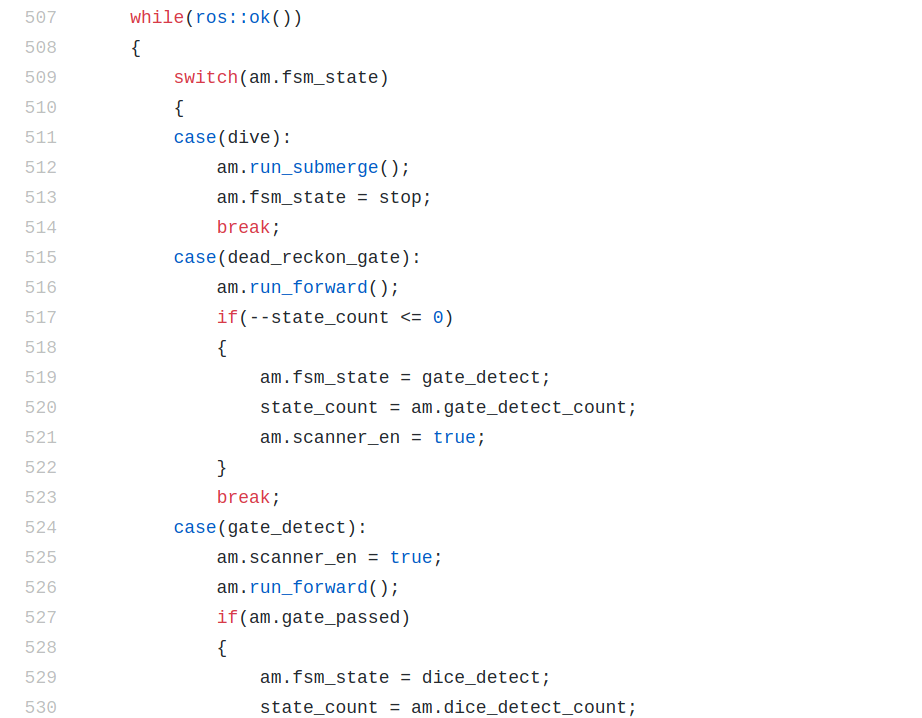
\includegraphics[width=150mm]{Figures/DirectStateHandling}
\decoRule
\caption[Direct State Handling]{Code segment showing the control systems way of handling states, controlling submarine functions, and getting information from other submarine systems.}
\label{fig:DirectStateHandling}
\end{figure}

The control system also directly handled the vision systems. The control system did offer a simple interface for the states in the state machine to utilize.

